\chapter{Wyniki i testy wydajnościowe}
\label{chap:research}

Ten rozdział zawiera zrzuty ekranu pokazujące wyrenderowane przykładowe sceny.
// HIRO więcej opis

\section{Przykładowe sceny}

Używane sceny zostały przygotowane na podstawie zebranych przez Khronos w repozytorium \cite{GLTFSAMPLEMODELS} następujących przykładowych modelów glTF przedstawiających:
\begin{itemize}
	\item \textit{MetalRoughSpheres}: różne wartości metalu i chropowatości materiałów używając sfer, patrz rys. \ref{screenshot_metalroughspheres};
	\item \textit{DamagedHelmet}: uszkodzony w walce hełm sci-fi, patrz rys. \ref{screenshot_damagedhelmet};
	\item \textit{Sponza}: wnętrze budynku inspirowane pałacem Sponza, często używane do testowania oświetlenia, patrz rys. \ref{screenshot_sponza}.
\end{itemize}

\begin{figure}[!htb]
	\centering
	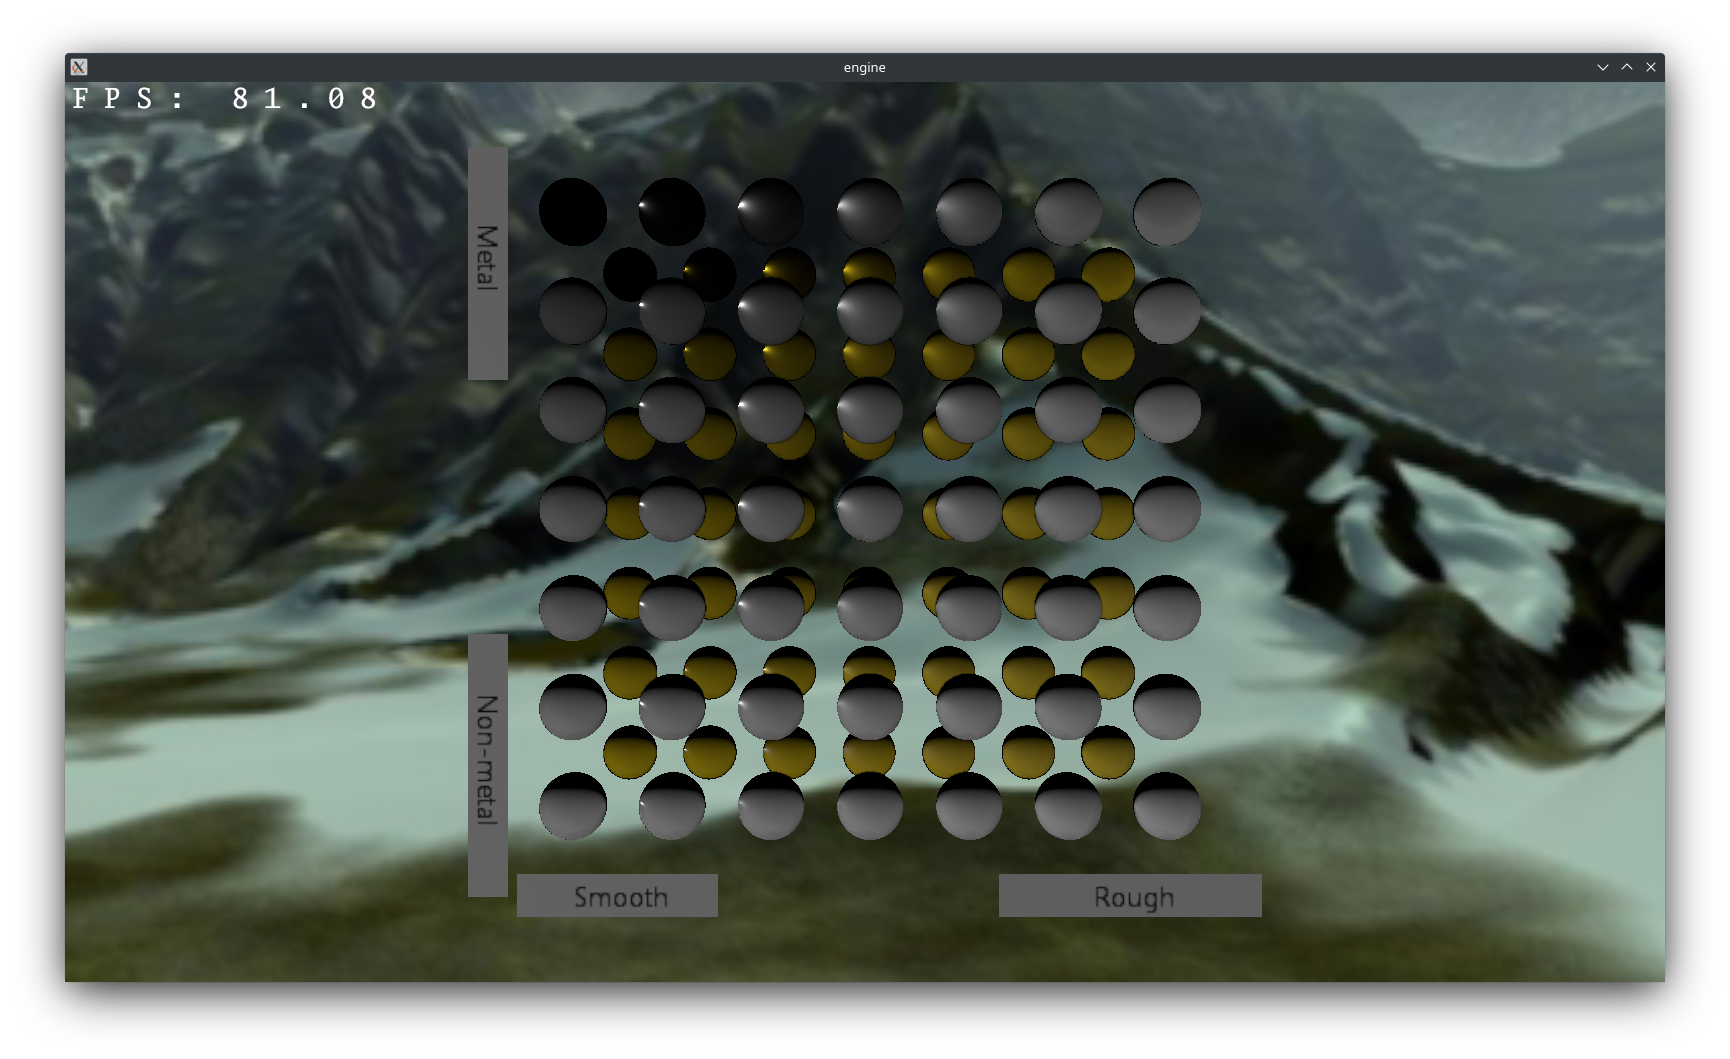
\includegraphics[width=0.8\textwidth]{images/render_metalroughspheres.png}
	\caption{Wynik renderowania sceny MetalRoughSpheres (opracowanie własne)}
	\label{screenshot_metalroughspheres}
\end{figure}

\begin{figure}[!htb]
	\centering
	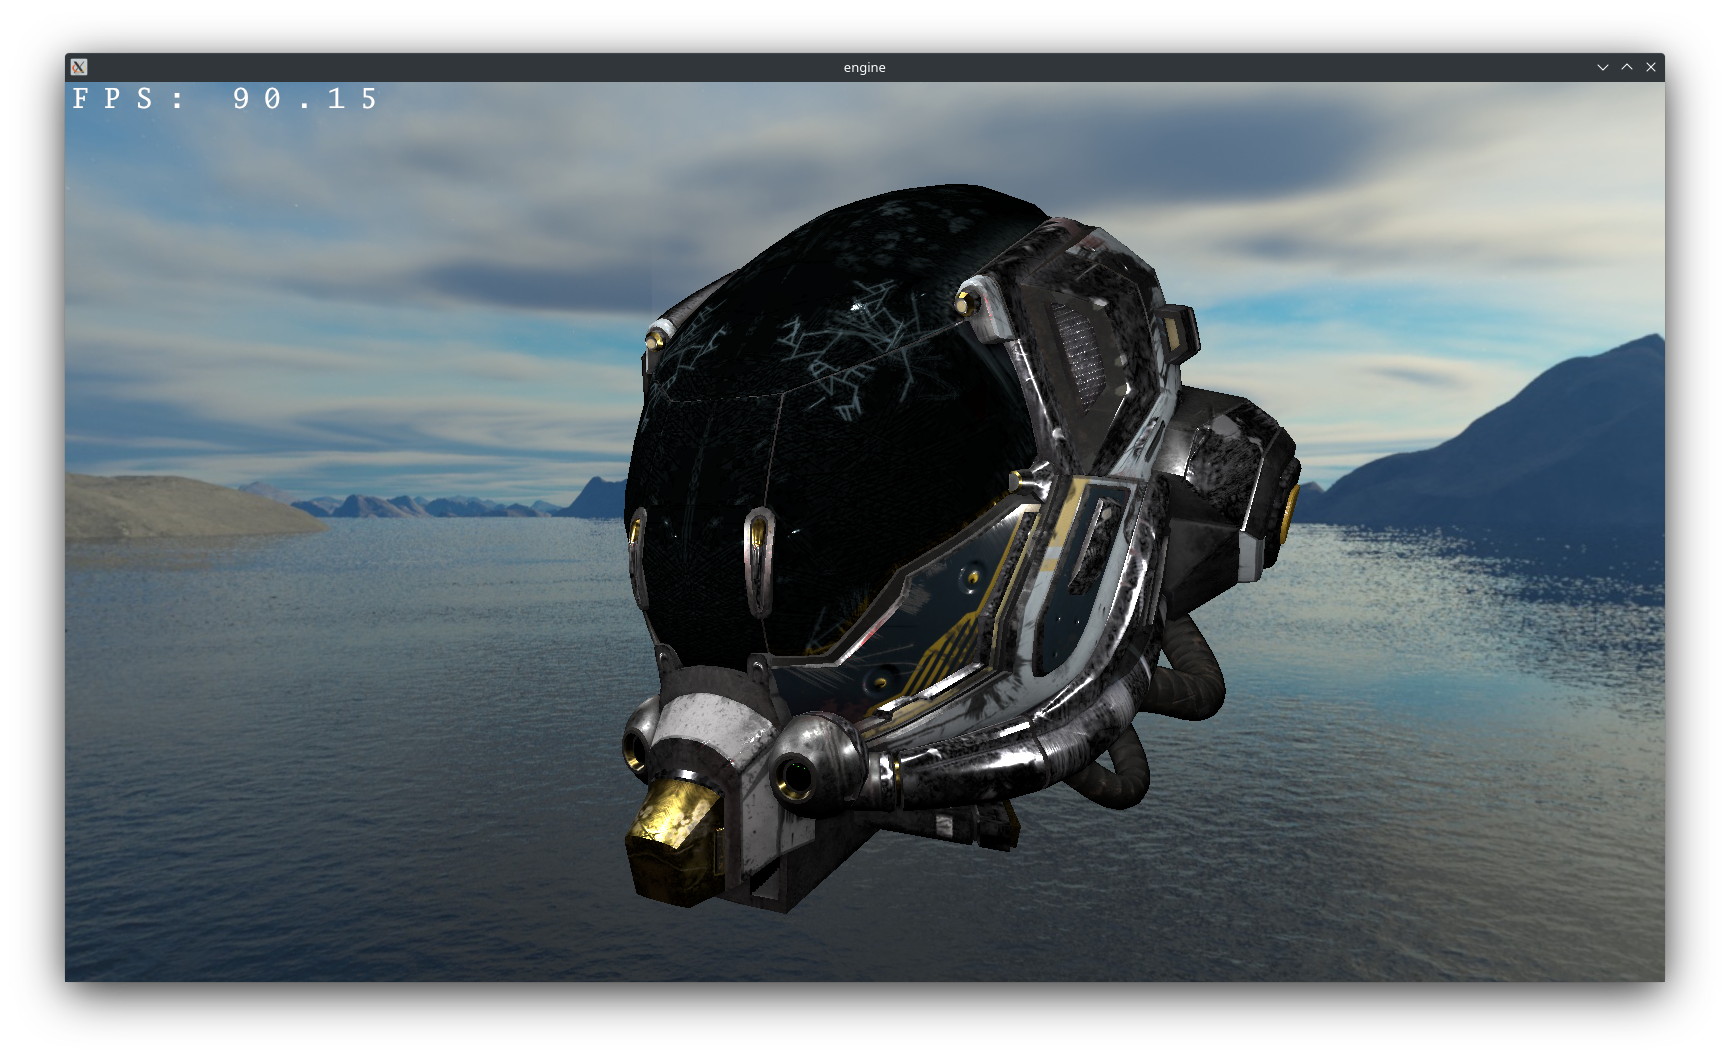
\includegraphics[width=0.8\textwidth]{images/render_damagedhelmet.png}
	\caption{Wynik renderowania sceny DamagedHelmet (opracowanie własne)}
	\label{screenshot_damagedhelmet}
\end{figure}

\begin{figure}[!htb]
	\centering
	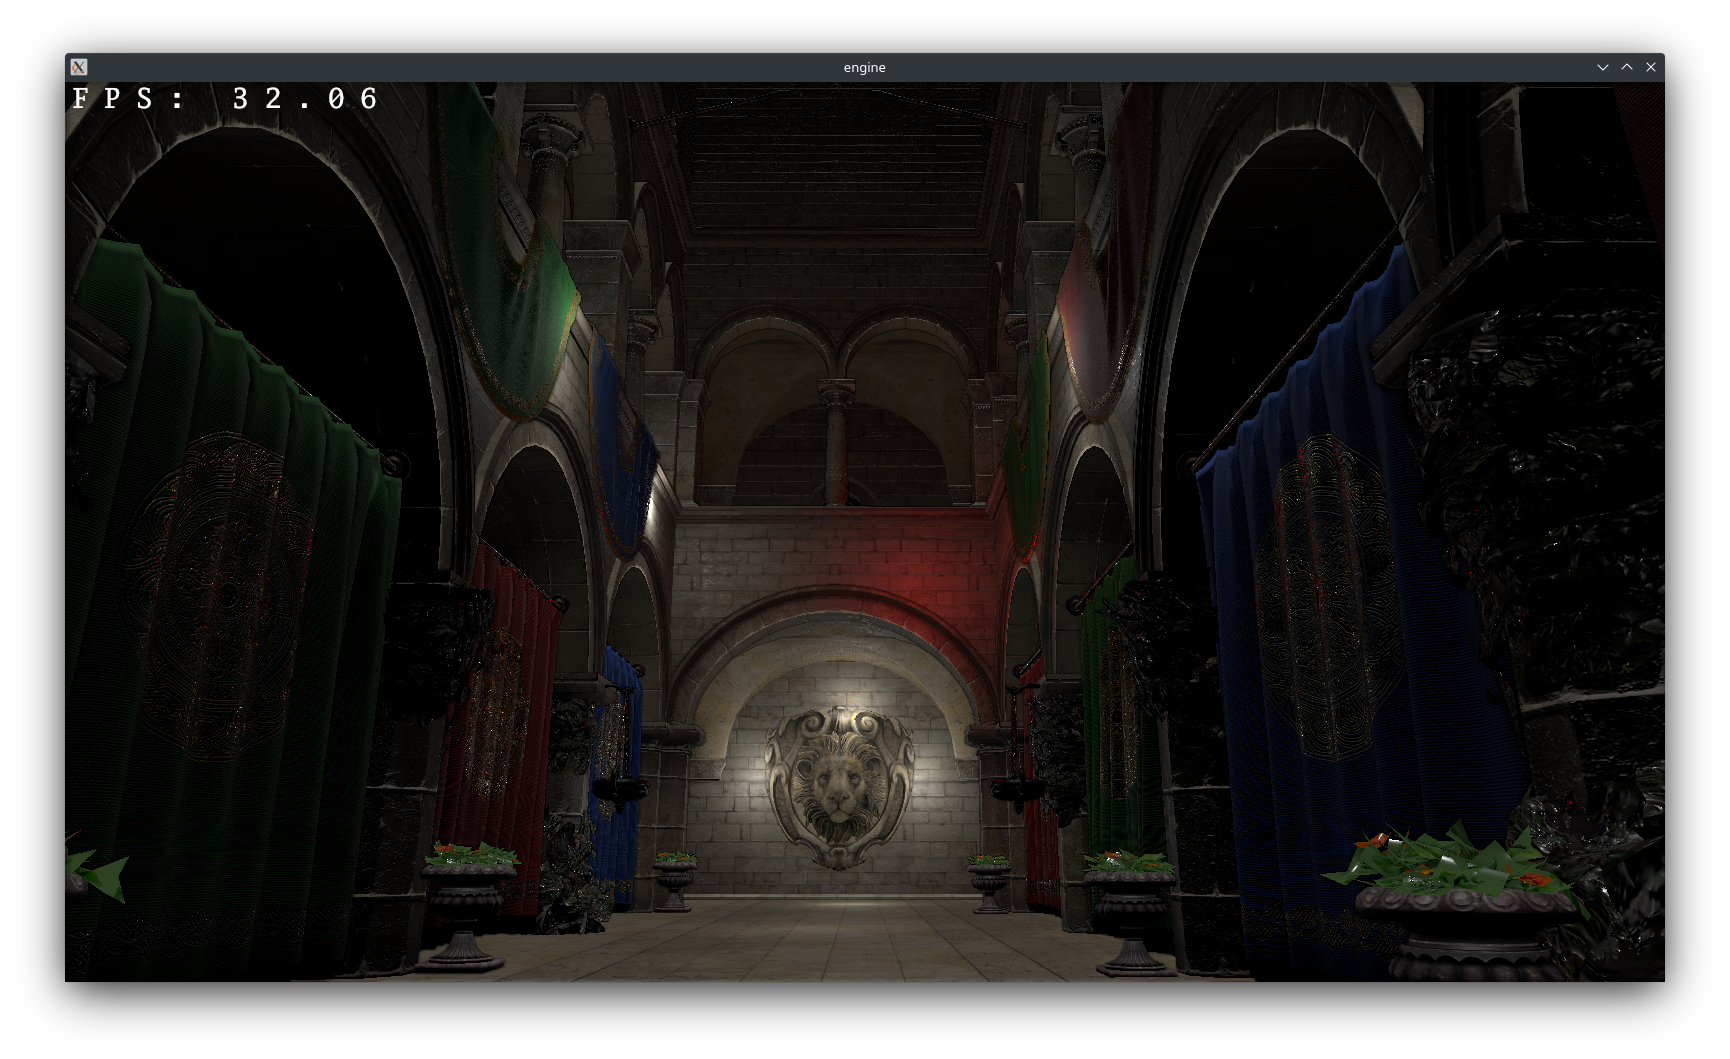
\includegraphics[width=0.8\textwidth]{images/render_sponza.png}
	\caption{Wynik renderowania sceny Sponza (opracowanie własne)}
	\label{screenshot_sponza}
\end{figure}

\section{Testy wydajnościowe}

// HIRO Profiling różne sceny. RENDERDOC counter, jak wpływa resolution?

// TODO: test: technika filtrowanie anizotropowe, usuń TRANSIENT
// TODO: test: usuń mipmapy, usuń multidraw
